\documentclass[14pt]{extarticle}

\begin{document}
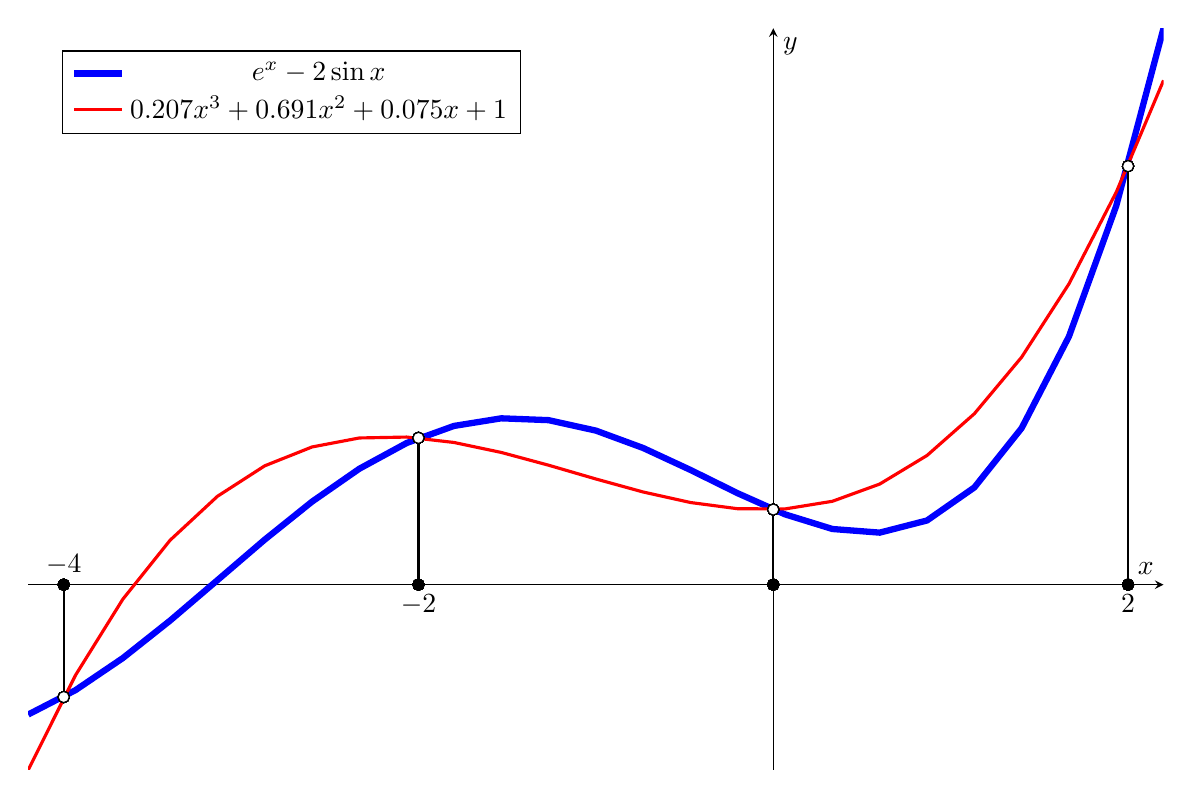
\begin{tikzpicture} [
	declare function= {
		u(\x) = e^\x - 2*sin(\x * 180 / pi);
		divDiff1(\a,\b) = (u(\b)-u(\a)) / (\b-\a);
		divDiff2(\a,\b,\c) = (divDiff1(\b,\c)-divDiff1(\a,\b)) /
			(\c-\a);
		divDiff3(\a,\b,\c,\d) = (divDiff2(\b,\c,\d) -
			divDiff2(\a,\b,\c)) / (\d-\a);
		newton(\x,\a,\b,\c,\d)= u(\a) + divDiff1(\a,\b)*(\x-\a)+
			divDiff2(\a,\b,\c)*(\x-\a)*(\x-\b) +
			divDiff3(\a,\b,\c,\d)*(\x-\a)*(\x-\b)*(\x-\c);
	},]
	\begin{axis} [
		height=11cm,
		width=16cm,
		xlabel = {$x$},
		ylabel = {$y$},
		axis x line = middle,
		axis y line = middle,
		domain = -4.2:2.2,
		ticks = none,
		legend pos = north west ]

		\newcommand*{\varA}{-4}
		\newcommand*{\varB}{-2}
		\newcommand*{\varC}{0}
		\newcommand*{\varD}{2}
		\pgfmathsetmacro{\fa}{u(\varA)}
		\pgfmathsetmacro{\fb}{u(\varB)}
		\pgfmathsetmacro{\fc}{u(\varC)}
		\pgfmathsetmacro{\fd}{u(\varD)}

		\addplot[color=blue, line width=.08cm]{u(x)};
		\addplot[color=red, line width=.04cm]{newton(x,\varA,
			\varB,\varC,\varD)};

		\coordinate(A) at 	(\varA,		\fa);
		\node[above](Ap) at	(\varA,		0) {$\varA$};
		\coordinate(B) at 	(\varB,		\fb);
		\node[below](Bp) at	(\varB,		0) {$\varB$};
		\coordinate(C) at 	(\varC,		\fc);
		\coordinate(Cp) at	(\varC,		0);
		\coordinate(D) at 	(\varD,		\fd);
		\node[below](Dp) at	(\varD,		0) {$\varD$};

		\addplot[mark=*,only marks, fill=white] (\varA,\fa)
			node[above, pos=1]{};
		\addplot[mark=*,only marks, fill=white] (\varB,\fb)
			node[above, pos=1]{};
		\addplot[mark=*,only marks, fill=white] (\varC,\fc)
			node[above, pos=1]{};
		\addplot[mark=*,only marks, fill=white] (\varD,\fd)
			node[above, pos=1]{};
		\addplot[mark=*,only marks, fill=black] (\varA,0)
			node[above, pos=1]{};
		\addplot[mark=*,only marks, fill=black] (\varB,0)
			node[above, pos=1]{};
		\addplot[mark=*,only marks, fill=black] (\varC,0)
			node[above, pos=1]{};
		\addplot[mark=*,only marks, fill=black] (\varD,0)
			node[above, pos=1]{};

		\draw[thick] (Ap) -- (A)	(Bp) -- (B)
			(Cp) -- (C)	(Dp) -- (D);

		\addlegendentry{$e^x-2\sin x$};
		\addlegendentry{$0.207x^3+0.691x^2+0.075x+1$};
	\end{axis}
\end{tikzpicture}
\end{document}
